\documentclass[a4paper,11pt]{article}
\usepackage{graphicx}
\usepackage{booktabs}
\usepackage{setspace}
\usepackage{parskip}
\onehalfspacing
\begin{document}

\author{Hiromasa Okada}
\title{\vspace{-2cm}Report for Sheet 4\\
\small{Lab Course Machine Learning and Data Analysis}}
\maketitle

\section*{Implementation comments}
In this exercise I implemented support vector machine and plot function of it. There are two type of support vector machines, the first one is trained by SMO algorithum and the second one is with direct solving of quadratic programming.

\begin{verbatim}
# SVM class with SMO algorithum
smo_svm = svm_smo(kernel, C, kernelparameter) 

# SVM class with quadratic problem
qb_svm=svm_qp(kernel, C, kernelparameter) 

\end{verbatim}

Both class get $kernel \in \{ 'gaussian','polynomial','linear' \}$ and C as a contraint parameter for lagrange multipliers. Both two classes has same kernel function "getkernel(self, X, Y=None)" and predict function "fx(self,X1,X2,Y)". 
On the other hands SMO class has following functions which QP class does not have.

\begin{verbatim}
_compute_box_constraints(self, i, j, Y, alpha, C)
_update_parameters(self, E_i, E_j, i, j, K, Y, alpha, b, C)
_compute_updated_b(self, E_i, E_j, i, j, K, Y, alpha_old, alpha_new, b_old, C)
\end{verbatim}

With these functions SMO class finds iteratively optimal lagrange multipliers and bias. But QP class solve quadratic programming in the function "fit(self, X, Y)" without functions above.
In both classes lagrange multipliers, bias, support vector and labels are saved as object like

\begin{verbatim}
self.SV= X[alp_idx]
self.y = Y[alp_idx]
self.alpha = self.alpha[alp_idx]
self.b = np.mean(self.y - self.fx(self.SV,self.SV,self.y)[:,0])
\end{verbatim}



\section*{Assignment 3}
The formular of the SVM optimization problem and the quadratic programming are given in 8th page of the slide.


\begin{figure}[htbp]
  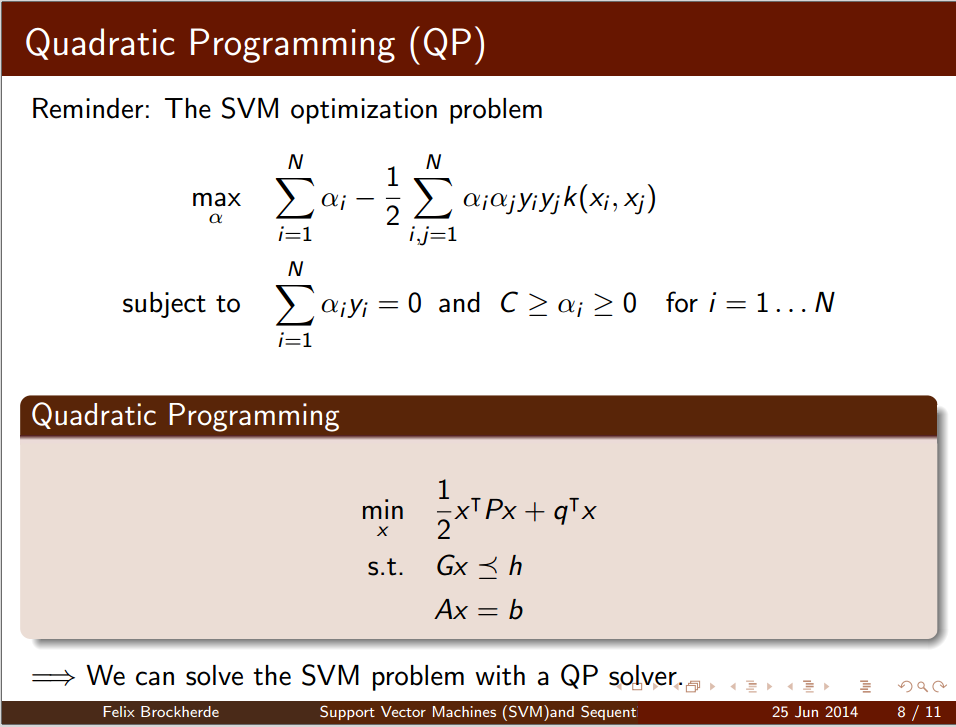
\includegraphics[scale=0.4]{qpform.png}
\end{figure}

The relation between them: 

\begin{eqnarray*}
\max_{\alpha} \:\:\:\:\:\:   \sum^N_{i=1} \alpha_i -\frac{1}{2} \sum^N_{i,j=1} \alpha_i \alpha_j y_i y_j k(x_i,x_j) \\
= \min_{\alpha} \:\:\:\:\:\:  -\sum^N_{i=1} \alpha_i +\frac{1}{2} \sum^N_{i,j=1} \alpha_i \alpha_j y_i y_j k(x_i,x_j)
\end{eqnarray*}
\begin{eqnarray*}
x= (\alpha_1,...,\alpha_N)^T, \:\: q=(-1,...-1)^T  
\end{eqnarray*}
\begin{eqnarray*}
P = Y \odot K, \:\:\:\:\:\: \mbox{Where} \odot \mbox{elementwise multiplication and }Y, K \in \mathbf{R}^{N \times N} \\
\end{eqnarray*}
\begin{eqnarray*}
Y = yy^T, \:\:\: y=(y_1,...y_i)^T \in \{ -1, 1\}^N, \:\:\:
K = 
\left(
\begin{array}{cccc}
k(x_1,x_1) & \cdots & k(x_1,x_j) \\
 \vdots & \ddots &  \vdots  \\
 k(x_i,x_1) & \cdots & k(x_i,x_j)
\end{array}
\right)
\end{eqnarray*}
\begin{eqnarray*}
G = 
\left[
\begin{array}{cccc}
-I \\
 I 
\end{array}
\right],  \:\:\:
h = 
\left(
\begin{array}{cccc}
0 \\
 \vdots  \\
0  \\
C \\
 \vdots  \\
C  \\
\end{array}
\right)
\:\:\:\: \mbox{Where } I \mbox{ is identical matrix and } G \in \mathbf{R}^{2N \times N}, \:\:\: h \in \mathbf{R}^{2N}
\end{eqnarray*}
\begin{eqnarray*}
A = (y_1,...,y_N) \in \mathbf{Z}^{1 \times N}, \:\: \forall_{i=0}^N \: y_i \in \{-1,1\}, \:\:\: b = [0] \in \mathbf{R}^{1 \times 1}
\end{eqnarray*}


\section*{Assignment 4}

\subsection*{1. Find parameters C and σ for a Gaussian kernel}
To find parameters C and σ for a Gaussian kernel I used the cross validation with following parameters

\begin{verbatim}
para = { 'kernel': ['gaussian'], 'kernelparameter': np.logspace(-2,2,10), 
		'regularization': np.linspace(1.0,3.0,10)}
\end{verbatim}

Then the parameters C and σ for a Gaussian kernel are

\begin{verbatim}
Kernelparameter:  0.599484250319
C:  2.77777777778
\end{verbatim}

After the plot of predictons of training data and test data I found that it classfied well and there was no over fitting and no under fitting by traing data so that it classfied also test data well.

\begin{verbatim}



\end{verbatim}


\begin{figure}[htbp]
  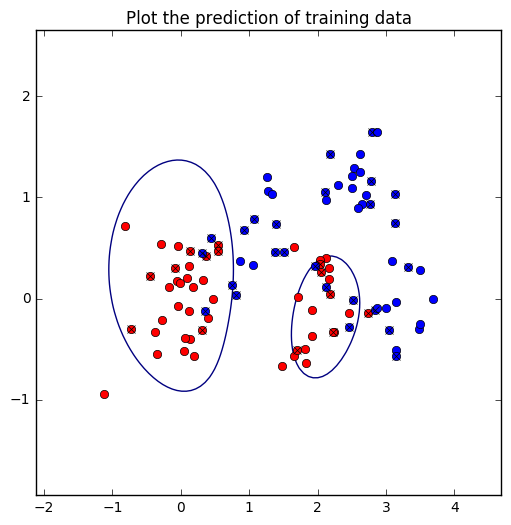
\includegraphics[scale=0.5]{trcvsmo.png}
  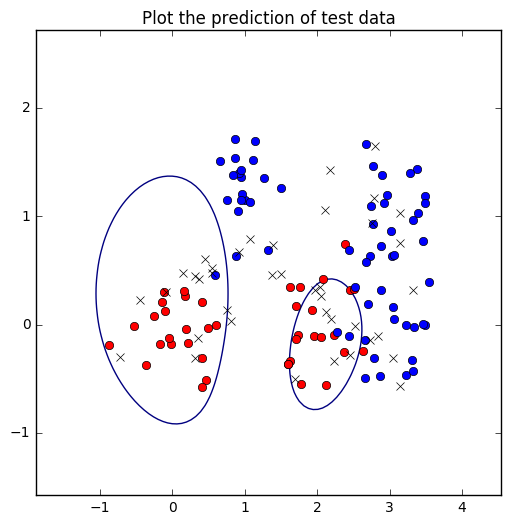
\includegraphics[scale=0.5]{tecvsmo.png}
\end{figure}

\subsection*{2. Over fitting and under fitting}
Which parameter C and σ for a Gaussian kernel overfit and underfit?
The parameters which cause underfitting are

\begin{verbatim}
Kernelparameter:  100.0
C:  0.7
\end{verbatim}

and plots are

\begin{figure}[htbp]
  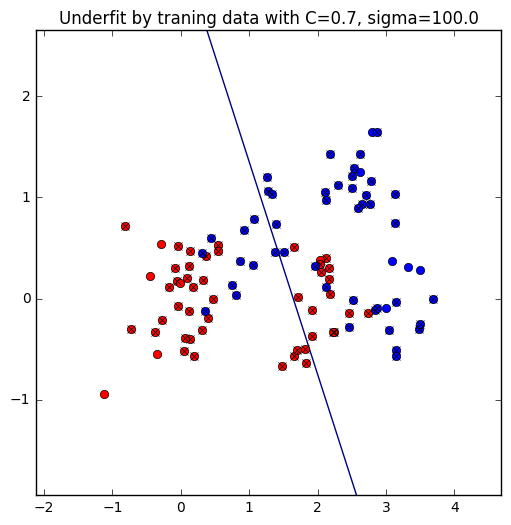
\includegraphics[scale=0.5]{smouftr.png}
  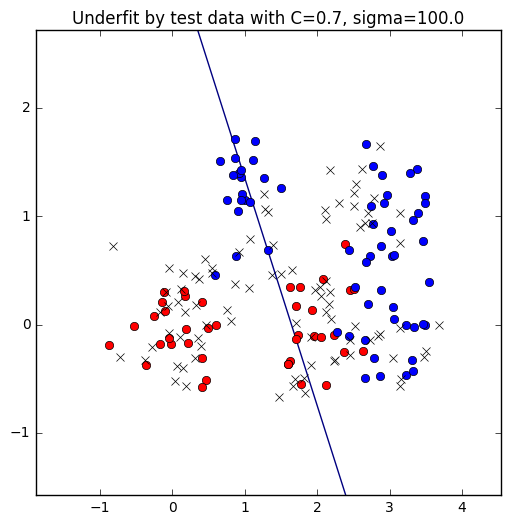
\includegraphics[scale=0.5]{smoufte.png}
\end{figure}

In case of the under fitting the classfier will be a linear.

\begin{verbatim}

\end{verbatim}

The parameters which cause overfitting are

\begin{verbatim}
Kernelparameter:  0.1
C:  3.7
\end{verbatim}

and plots are

\begin{figure}[htbp]
  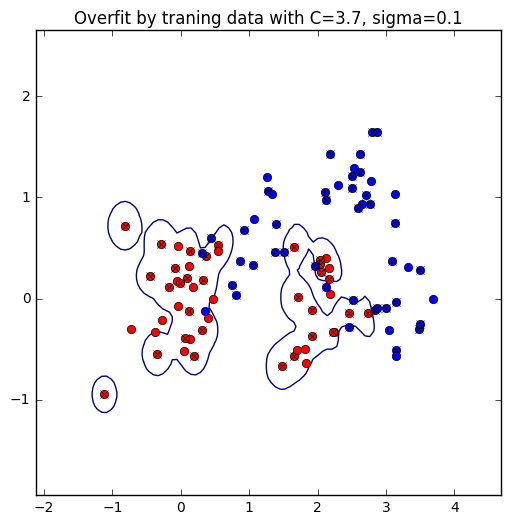
\includegraphics[scale=0.5]{smooftr.png}
  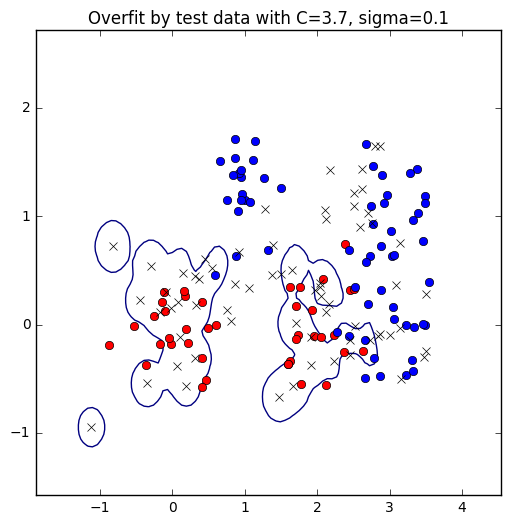
\includegraphics[scale=0.5]{smoofte.png}
\end{figure}

In case of the overfitting there are more than two clusters even we don't need more.
When the sigma is higher and C is lower than optimal it tends to underfit, on the other hands the sigma is lower and C is higher than optimal it tends to overfit.

\subsection*{3. ROC curve with different bias}

For optimal C and $\sigma$, a receiver operator characteristics (ROC) curve is plotted by varying the bias
parameter b of your SVM model. 

\begin{figure}[htbp]
  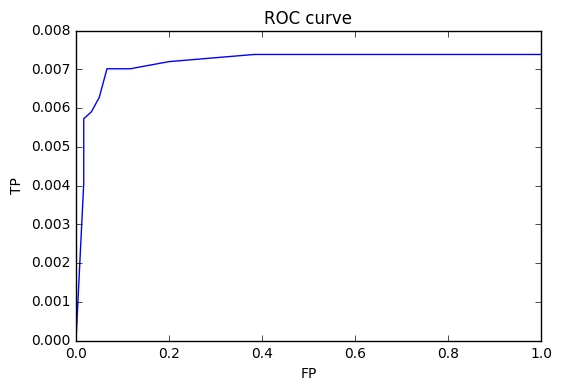
\includegraphics[scale=0.5]{roc.png}
\end{figure}

The used possible bais are in this range:

\begin{verbatim}
bias = np.linspace(-10,10,110)
\end{verbatim}


\section*{Assignment 5}

\section*{Assignment 6}

\section*{Assignment 7}



\end{document}

